
\noindent\mnDifficult
\begin{slikaDesno}{fig/RC.pdf}
    \PID 
    У колу приказаном на слици познати су $R$ и $C$. Облик напона напонског генератора је 
    униполарна поворка правоугаоних импулса, која почиње у тренутку $t=0$, 
    а која је дефинисана у задатку \ref{z:snaga_pwm}, а познати су $V_{\rm m}$, $0 \leq D \leq 1$ и $T$. 
    (а) Ако је $n \geq 0$ број протеклих периода побудног напона, одредити диференцну једначину за излазни напон 
    $\Upphi(v_{\rm I}[n], v_{\rm I}[n+1])$ преко задатих параметара.
    (б) Ако је $v_{\rm I}[0] = 0$, одредити излазни напон $v_{\rm I}[n]$, где је $n$ број протеклих периода улазног сигнала.     
\end{slikaDesno} \\[5mm]

\RESENJE

    Одредити (в) импулсни одзив
Задатак се може решити применом Лапласове и $\mathcal{Z}$-трансформације. Лапласовом трансформацијом се разматра понашање система током једног периода, 
док се $\mathcal{Z}$-трансформацијом ти различити периоди повезују. Посматрамо време $0 < t < T$ након $n$ периода улазног напона, у оквиру тога 
сматрамо да је $v_{\rm I}[n]$ позната величина док $v_{\rm I}[n+1]$ треба одредити. Применом заменске шеме за кондензатор, као и заменом уопштених 
комплексних импеданси коло се може поједноставити. Такво коло онда представља уопштени напонски разделник па је онда 
\begin{eqnarray}
    V_{\rm I}(s) = \dfrac{v_{\rm I}[n] R + V_{\rm G}(s) \dfrac{1}{sC}}{R + \dfrac{1}{sC}} = 
    \dfrac{v_{\rm I}[n] sRC + V_{\rm G}(s) }{sRC + 1} = \dfrac{v_{\rm I}[n] s \uptau + V_{\rm G}(s) }{s\uptau + 1},
\end{eqnarray}
при чему је уведен параметар $\uptau = RC$ као временска константа система. Лапласова трансформација побудног напона је 
$V_{\rm G} = V_{\rm m}\dfrac{1 - \ee^{-sDT}}{s}$, па се заменом добија 
\begin{eqnarray}
    V_{\rm I}(s) = \dfrac{v_{\rm I}[n] s \uptau + V_{\rm m}\dfrac{1 - \ee^{-sDT}}{s} }{s\uptau + 1} =
       \dfrac{v_{\rm I}[n] s \uptau }{s \uptau + 1} +
       \dfrac{V_{\rm m}\left(1 - \ee^{-sDT}\right) }{s(s\uptau + 1)}, \label{eq:\ID.2}
\end{eqnarray}
Растављањем на парцијалне разломке, као у додатку \ref{a:pfd}, други сабирак се може расписати као  
\begin{eqnarray}
    V_{\rm I}(s) = 
    V_{\rm m} \left(1 - \ee^{-sDT}\right) \dfrac{ 1 }{s(s\uptau + 1)} 
    = 
    V_{\rm m} \left(1 - \ee^{-sDT}\right) \left(\dfrac{1}{s} - \dfrac{1}{s + \uptau^{-1}} \right).
\end{eqnarray}
Заменом добијеног резултата у \eqref{eq:\ID.2}, па одређивањем инверзне Лапласове трансформације, се налази резулат у временском домену
\begin{eqnarray}
    v_{\rm I}(t) &=& \ILT{V_{\rm I}(s)} \\
    &=& 
    v _{\rm I}[n] \ee^{-t/\uptau} \uu(t)
    +
    V_{\rm m}(1 - \ee^{-t/\uptau}) \uu(t)
    -
    V_{\rm m}(1 - \ee^{-(t-DT)/\uptau}) \uu(t-DT).
\end{eqnarray}
За успостављање тражене диференцне везе, релевантна је вредност $v_{\rm I}(t = T) = v_{\rm I}[n+1]$, па се заменом има
\begin{eqnarray}
    v_{\rm I}(T)
    &=&
    v _{\rm I}[n] \ee^{-T/\uptau} \cancelto{1}{\uu(T)}
    +
    V_{\rm m}(1 - \ee^{-T/\uptau}) \cancelto{1}{\uu(T)}
    -
    V_{\rm m}(1 - \ee^{-(1-D)T/\uptau}) \cancelto{1}{\uu((1-D)T)}
    \\
    &=&
    v _{\rm I}[n] \ee^{-T/\uptau}
    +
    V_{\rm m}(1 - \ee^{-T/\uptau})
    -
    V_{\rm m}(1 - \ee^{-(1-D)T/\uptau})
    \\ 
    &=&
    v _{\rm I}[n] \ee^{-T/\uptau}
    +
    V_{\rm m}
    \left(
         \ee^{-(1-D)T/\uptau} - \ee^{-T/\uptau}
    \right).
\end{eqnarray}
Тражена диференцна једначина се онда може записати у облику 
\begin{eqnarray}
    v_{\rm I}[n+1] 
    = 
    \upalpha v_{\rm I}[n]
    + 
    \upbeta V_{\rm m}, \quad
    \text{где су}
    \quad
    \upalpha = \ee^{-T/\uptau}, 
    \quad
    \upbeta =  \ee^{-(1-D)T/\uptau} - \ee^{-T/\uptau}. \label{\ID.3}
\end{eqnarray}


\begin{figure}[b!]
    \centering
    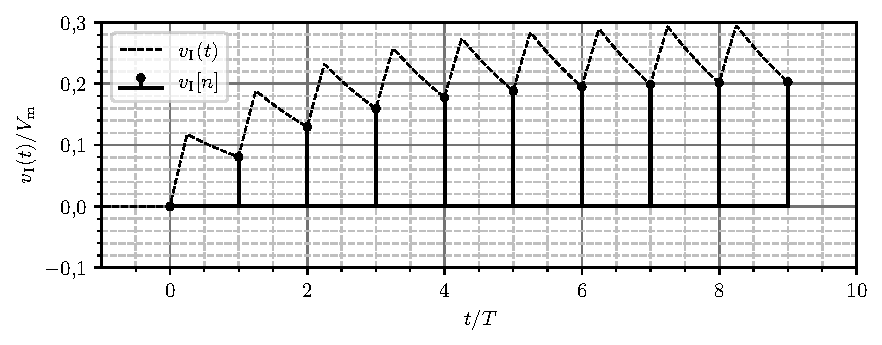
\includegraphics{fig/zt_pwm.pdf}
    \caption{Уз резултат задатка, $T/\uptau = 2$, $D = 25\%$, приказан је континуални резултат, као и низ добијен као резултат задатка.} 
    \label{fig:\ID.3}
\end{figure}
%
(б) Диференцна једначина добијена у \eqref{\ID.3} може се решити применом $\mathcal{Z}$-трансформације према: 
\begin{eqnarray}
    \ZT{v_{\rm I}[n+1]} &=& \upalpha \ZT{v_{\rm I}[n]} + \upbeta \ZT{V_{\rm m}} \\ 
    z V_{\rm I}(z) - \cancelto{0}{zv_{\rm I}[0]}
    &=&  
    \upalpha V_{\rm I}(z) + \dfrac{\upbeta V_{\rm m} z}{z-1}.
\end{eqnarray}
Решавањем добијене једнакости по $V_{\rm I}(z)$ па применом инверзне $\mathcal{Z}$-трансформације налази се 
\begin{eqnarray}
    V_{\rm I}(z) = \dfrac{
        \upbeta V_{\rm m} z
    }{(z - 1)(z - \upalpha)} 
    \Rightarrow
    v_{\rm I}[n] = \IZT{V_{\rm I}(z)} =
    \upbeta V_{\rm m} \dfrac{\upalpha^n - 1}{\upalpha - 1} \uu[n].
\end{eqnarray}
Добијени резултат је илустрован на слици \ref{fig:\ID.3} за један одабрани конкретан сет параметара. Такође, примећује се да је облик 
сигнала одзива завистан само од параметара $T/\uptau$. 

